% TeX encoding = utf8
% TeX spellcheck = pl_PL 
\documentclass[a4paper, 11pt]{article}
\usepackage[utf8]{inputenc}
\usepackage[polish]{babel}
\usepackage{polski}
\usepackage{graphicx}
\usepackage{listings}
\usepackage{amsfonts}
\usepackage{geometry}
\usepackage{multicol}
\usepackage{latexsym}
\usepackage{enumerate}
\usepackage{hyperref}
\usepackage{wrapfig}
\usepackage{color} %red, green, blue, yellow, cyan, magenta, black, white
\definecolor{mygreen}{RGB}{28,172,0} % color values Red, Green, Blue
\definecolor{mylilas}{RGB}{170,55,241}

\author{Kamil Foryszewski}
\title{Dokumentacja projektu laboratoryjnego numer 2 przedmiot MNUM}
\frenchspacing

\newgeometry{tmargin=2cm, bmargin=2cm, lmargin=2cm, rmargin=2cm}
\pagestyle{empty}


\begin{document}

\lstset{language=Matlab,%
    basicstyle=\color{red},
    breaklines=true,%
    morekeywords={matlab2tikz},
    keywordstyle=\color{blue},%
    morekeywords=[2]{1}, keywordstyle=[2]{\color{black}},
    identifierstyle=\color{black},%
    stringstyle=\color{mylilas},%
    commentstyle=\color{mygreen},%
    showstringspaces=false,
    numbers=right,%
    numberstyle={ \color{black}},% size of the numbers
    numbersep=5pt, % this defines how far the numbers are from the text
    emph=[1]{for,endfor,endwhile,endfunction,endif,break},emphstyle=[1]\color{blue}, %some words to emphasise
    emph=[2]{,.}, emphstyle=[2]\color{yellow},%
}

\maketitle
\tableofcontents

\section{Zadanie 1}

\subsection{Polecenie}
Proszę napisać program służący do obliczania wartości własnych macierzy nieosobliwych metodą rozkładu QR w dwóch wersjach: bez przesunięć i z przesunięciami dla macierzy symetrycznej oraz z przesunięciami dla macierzy niesymetrycznej. Następnie proszę przetestować skuteczoność (zbieżność obu wersji algorytmu dla 30 różnych macierzy losowych o wymiarach 5x5, 10x10 i 20x20. Proszę podać średnią liczbę iteracji dla obu metod. Dla wybranych macierzy proszę porównać otrzymane wyniki z wartościami własnymi obliczonymi poleceniem eig(). 

\subsection{Rozkład QR}
\subsubsection{Opis teoretyczny}
Rozkład QR macierzy kwadratowej A polega na tym aby macierz $A$ zapisać w postaci iloczynu $QR$, gdzie macierz $Q$ jest macierzą ortogonalną, a $R$ jest macierzą trójkątną górną. Macierz $Q$ o wyrazach rzeczywistych nazywamy ortogonalną, jeżeli spełnia warunek $QQ^T = I$. Rozkład QR można uzyskać stosując różne algorytmy zależne od wyboru przekształceń. Jeżeli założymy, że macierz $A$ jest nieosobliwa i że na przekątnej macierzy $R$ są wyrazy dodatnie, to rozkład jest jednoznaczny, a  więc  nie  zależy  od  wyboru  algorytmu.

\subsubsection{Metoda Gramma-Schmidta}
$A \in \mathbb{R}^{m,n}$ jest macierzą o liniowo niezależnych kolumnach $\vec a_1, \dots, \vec a_n \in \mathbb{R}^n$.  Przeprowadzając ortogonalizację Grama-Schmidta tych kolumn, otrzymujemy ortonormalny układ wektorów $\vec q_1, \dots, \vec q_n$ 
\\
\\
$\vec b_k = \vec a_k - \sum_{j=1}^{k-1} (\vec q_j^T \vec a_k ) \vec q_j, 
    \quad \vec q_k = \|\vec b_k\|_2^{-1} \vec b_k, \qquad k = 1,2, \dots, n.$
\\
\\
Niech
\\
\\
$r_{j,k} = \vec q_j^T \vec a_k, \quad (j = 1, \dots, k - 1), \qquad r_{k,k} = \| \vec b_k \|_2,
        \qquad  r_{j,k} = 0, \quad (j > k)$
\\
\\
i
\\
\\
$Q = [\vec q_1, \dots, \vec q_n ] \in \mathbb{R}^{m,n}, \qquad R = [r_{i,j}] \in \mathbb{R}^{n,n}.$
\\
\\
Wtedy $Q$ jest macierzą o ortogonalnych kolumnach, $R$ jest macierzą trójkątną górną i $A = QR$.
Ponieważ wyżej przedstawiona medota ma gorsze własności numeryczne od tzw. zmodyfikowanej metody Gramma-Schmidta, to na potrzeby realizacji zadania zostanie użyta metoda o lepszych własnościach numerycznych. Modyfikacja polega na zmianie kolejności ortogonalizacji. Zamiast ortogonalizować kolumny po kolei, algorytm najpierw wyznacza współczynnik dla pierwszej kolumny a następnie ortogonalizuje względem niego pozostałe. 

\subsubsection{Realizacja w programie Matlab}
\begin{lstlisting}
%funkcja rozkladu qr macierzy zmodyfikowanym algorytmem Grama-Schmidta
%Na podstawie ksiazki prof. Tatjewskiego
function [Q,R] = qrgsm(A)

  [m n] = size(A);
  Q = zeros(m,n);
  R = zeros(n,n);
  d = zeros(1,n); 
  %rozklad A kolumnowo ortogonalny
  for i=1:n
    Q(:,i) = A(:,i);
    R(i,i) = 1; 
    d(i) = Q(:,i)'*Q(:,i);
    for j=i+1:n
      R(i,j) = (Q(:,i)'*A(:,j))/d(i);
      A(:,j) = A(:,j)-R(i,j)*Q(:,i);  
    end 
  end
  %normowanie
  for i=1:n
    dd = norm(Q(:,i));
    Q(:,i) = Q(:,i)/dd;
    R(i,i:n) = R(i,i:n)*dd;
  end
  
end 

\end{lstlisting}

\subsection{Znajdowanie wartości własnych metodą QR bez przesunięć}
\subsubsection{Opis teoretyczny}
Jedną z metod wyznaczania wartości własnych macierzy jest metoda wykorzystująca rozkład QR macierzy. 
Metoda ta w najprostszym wariancie ma następującą postać:
\\
\\
\hspace{8cm}$A_{0} := A; Z_{0} := I;$
\\
\hspace{8cm}dla $k = 1,2,3...$
$$
\left\{ \begin{array}{ll}
A_{k-1} := Q_{k}R_{k};\\
A_{k} := R_{k}Q_{k}; & \\
Z_{k} := Z{k-1}Q_{k};& \\
\end{array} \right.
$$

\subsubsection{Realizacja w programie Matlab}
\begin{lstlisting}
%funkcja wyznaczjaca wartosci wlasne metoda qr bez przesuniec
%na podstawie ksiazki prof. Tatjewskiego
function [D,t,i,v] = eignoshift (A, prec, it)

  s = tic;
  v=1;
  n = size(A,1); 
  i = 1; 
  while i <= it && max(max(A-diag(diag(A)))) > prec
    [Q1,R1] = qrgsm(A);
    A = R1*Q1; 
    i = i + 1;
  end
  if i > it 
    %error('przekrczono maksymalna liczbe iteracji');
    v=0;
  end
  D = diag(A);  
  t = toc(s);

end
\end{lstlisting}

\subsubsection{Zbieżność metory QR}
Dla macierzy $A$ symetrycznej macierz $A_{k}$ zbiega do macierzy diagonalnej $diag(\lambda_{i})$. Szybkość zbierzonosći przedstawia następujący wzór:
\\
\\
$\frac{|a_{i+1,i}^{k+1}|}{|a_{i+1,i}^{k}|} \approx |\frac{\lambda_{i+1}}{\lambda_{i}}|$
\\
\\
Z którego wynika że jeżeli wartości własne leżą blisko siebie to metoda powoli zbiega do rozwiązania. Aby poprawić jej zbierzność stosuje się zmodywikowaną metodę, którą opiszę poniżej. 

\subsection{Metoda QR z przesunięciami}
\subsubsection{Opis teoretyczny}
Metodę wyznaczania wartości własnych QR z przesunięiami można przybliżyć poniższym algorytmem:

\begin{enumerate}
  \item Znajdujemy wartość własną $\lambda_{n}$ jako najbliższą wartość własną podmacierzy 2x2 z prawego dolnego rogu macierzy $A^{(k)}$ wyznaczając wartości własne jako pierwiastki wielomianu drugiego stopnia o współczynnikach wielomianu charakterystycznego. 
  \item Opuszczamy ostatni wiersz i ostatnią kolumnę aktualnej macierzy $A^{(k)}$ (deflacja).
  \item Znajdujemy następną wartość własną $\lambda_{n-1}$, przekształcając macierz $A_{n-1}^{(k)}$ aż do uzyskania $e_{n-2}^{(k)} = 0$. Iterujemy aż do wyzerowania wszystkich elementów poza elementem diagonalnym (pętla while). 
  \item Powtarzamy kroki 2 i 3 aż do uzyskania wszystkich wartości własnych uwzględniając oczekiwaną prezycję obliczeń. 
\end{enumerate} 

\subsubsection{Realizacja w programie Matlab}
\begin{lstlisting}
%funkcja zwracajaca diagonalna maciez z wartosciami wlasnymi metoda qr z przesunieciami 
%A macierz wejsciowa , prec prezycja wyniku, it maksymalna liczba iteracji
%Na podstawie skryptu prof. Tatjewskiego
function [D,t,iteration,v] = eigshift (A, prec, it)

  n = size(A,1);
  D = diag(zeros(n));
  I = A; %macierz poczatkowa
  v = 1; 
  iteration = 0;
  time = tic;
  for k=n:-1:2
    K = I(1:k, 1:k); % macierz poczatkowa dla pojedynczej wart. wlasnej
    i=0; 
    while i <= it && max(abs(K(k,1:k-1))) > prec
      p = [1 -(K(k-1,k-1)+K(k,k)) K(k,k)*K(k-1,k-1)-K(k,k-1)*K(k-1,k)];
      ev = roots(p);
      % M = [a b,c d] rownanie dla M : 1*x^2 -(a+d)*x +a*d-c*b
      if abs(ev(1)-K(k,k)) < abs(ev(2)-K(k,k))
        shift = ev(1); %bajblizsza wartosc wlasna podmacierzy DD
      else
        shift = ev(2); 
      end
      K = K-eye(k)*shift; %przesuniecie macierzy
      [Q,R] = qrgsm(K); 
      K = R*Q+eye(k)*shift; % przeksztaucenie macierzy
      i = i+1;
      iteration = iteration +1;
    end
    if i>it
      %error('przekroczono maksymalna liczbe iteracji');
      v = 0; 
      break;
    end
    D(k) = K(k,k);
    if k>2
      I = K(1:k-1,1:k-1); %deflacja macierzy
    else
      D(1) = K(1,1); %ostatnia wartosc wlasna
    end
  end
  t = toc(time);
  
end

\end{lstlisting}

\subsection{Uwarunkowanie danych z zadania}
W zadaniu dane są macierze zarówno symetryczne jak i niesymetryczne generowane losowo przez wbudowaną funkcję rand(). Dla macierzy rzeczywistych i symetrycznych zachodzi twierdzenie Bauera-Frike'a mówiące wprost że $cond(X) = 1$ gdzie $X$ jest symetyczna o wartościach rzeczywistych. Z kolei dla macierzy niediagonalizowalnych uwarunkowanie wartości może być dowolnie duże, co również wynika z twierdzenia. 

\subsection{Skrypt generujący rozwiązanie zadania w programie Matlab}
\begin{lstlisting}
%realizacja zadania 1 z projektu 2.17
  clear; 
  F = fopen('results.txt','w'); %wynik zapisany do pliku
  fprintf(F, 'Wyniki do zadania numer 1 \n');
  Z = [5 10 20];
  
  %macierz symetryczna
  fprintf(F, '<<<Macierz symetryczna>>>\n\n');
  for i=1:3;
    Gtimen = 0; %zmienne do wyliczania srednich wartosci
    Gitern = 0; 
    Gprecn = 0; 
    Gvalidn = 0; 
    Gtimes = 0; 
    Giters = 0; 
    Gprecs = 0; 
    Gvalids = 0;
    Gteig = 0; 
    for j=1:30
      A = cmsim(Z(i));
      [R,timen,itn,validn] = eignoshift(A,0.00001,1000);% metoda bez przesuniec
      [S,times,its,valids] = eigshift(A,0.00001,1000); % metoda z przesunieciami
      eigstart = tic; 
      E = eig(A);
      teig = toc(eigstart);
      Gteig = Gteig + teig;
      Gtimen = Gtimen + timen;
      Gitern = Gitern + itn; 
      Gprecn = Gprecn + norm(R-E);
      if validn == 1
        Gvalidn = Gvalidn + 1; % zliczanie poprawnych rozwiazan
      end
      Gtimes = Gtimes + times;
      Giters = Giters + its; 
      Gprecs = Gprecs + norm(S-E);
      if valids == 1 
        Gvalids = Gvalids + 1;
      end
    end
    Gtimen = Gtimen/Gvalidn; 
    Gitern = Gitern/Gvalidn;      
    Gprecn = Gprecn/Gvalidn;
    Gtimes = Gtimes/Gvalids; 
    Giters = Giters/Gvalids;
    Gprecs = Gprecs/Gvalids;
    Gteig = Gteig/30; 
    fprintf(F, '<<<Liczba rownan %d >>>\n',Z(i));
    fprintf(F, '<<<Macierz symetryczna bez przesuniec>>>\n');
    fprintf(F, 'Sredni czas wykonania: %d\n',Gtimen);
    fprintf(F, 'Srednia ilosc iteracji: %d\n',Gitern);
    fprintf(F, 'Ilosc zakonczonych: %d\n',Gvalidn);
    fprintf(F, 'Srednia roznica miedzy eig(): %d\n\n',Gprecn);
    
    fprintf(F, '<<<Macierz symetryczna z przesunieciami>>>\n');
    fprintf(F, 'Sredni czas wykonania: %d\n',Gtimes);
    fprintf(F, 'Srednia ilosc iteracji: %d\n',Giters);
    fprintf(F, 'Ilosc zakonczonych: %d\n',Gvalids);
    fprintf(F, 'Srednia roznica miedzy eig(): %d\n\n',Gprecs);
    
    fprintf(F, '<<<Wyniki dla funkcji eig()>>>\n');
    fprintf(F, 'Sredni czas wykonania: %d\n',Gteig);
  end
  % macierz niesymetryczna
  fprintf(F, '<<<Macierz niesymetryczna>>>\n\n');
  for i=1:3;
    Gtimes = 0; 
    Giters = 0; 
    Gprecs = 0; 
    Gvalids = 0;
    Gteig = 0;  
    for j=1:30
      A = cmunsim(Z(i)); 
      [S,times,its,valids] = eigshift(A,0.00001,1000);
      eigstart = tic; 
      E = eig(A);
      teig = toc(eigstart);
      Gteig = Gteig + teig;
      if valids == 1
        Gtimes = Gtimes + times; 
        Giters = Giters + its; 
        Gprecs = Gprecs + norm(S-E); 
        Gvalids = Gvalids + 1;
      end
    end
    Gtimes = Gtimes/Gvalids; 
    Giters = Giters/Gvalids;
    Gprecs = Gprecs/Gvalids;
    Gteig = Gteig/30; 
    
    fprintf(F, '<<<Liczba rownan %d >>>\n',Z(i));
    fprintf(F, '<<<Macierz niesymetryczna z przesunieciami>>>\n');
    fprintf(F, 'Sredni czas wykonania: %d\n',Gtimes);
    fprintf(F, 'Srednia ilosc iteracji: %d\n',Giters);
    fprintf(F, 'Ilosc zakonczonych: %d\n',Gvalids);
    fprintf(F, 'Srednia roznica miedzy eig(): %d\n\n',Gprecs);
    
    fprintf(F, '<<<Wyniki dla funkcji eig()>>>\n');
    fprintf(F, 'Sredni czas wykonania: %d\n',Gteig);
  end
  
  fclose(F);
   
\end{lstlisting}
\vspace{1cm}


\subsection{Wyniki}
Wyniki w postaci tabularycznej wygenerowane przez powyższy skrypt:\\

\begin{table}[h]
\centering
\caption{Wyniki dla macierzy symetrycznych}
\begin{tabular}{|l|l|l|l|l|l|}
\hline
\textbf{Rozmiar} & \textbf{Funkcja} & \textbf{Czas (s)} & \textbf{Ilość Iteracji} & \textbf{Ilość zakończonych}
& \textbf{Różnica eig()}\\ \hline
5x5     & bez przesunięć   & 0.0619796   & 62.1333        & 30                 & 7.95247       \\ \hline
5x5     & z przesunięciami & 0.00865486  & 7.96667        & 30                 & 7.48066       \\ \hline
5x5     & eig()            & 3.31163e-05 & -              & 30                 & -             \\ \hline
10x10   & bez przesunięć   & 0.773586    & 256.321        & 28                 & 17.7433       \\ \hline
10x10   & z przesunięciami & 0.0323579   & 14.5333        & 30                 & 15.7378       \\ \hline
10x10   & eig()            & 4.24306e-05 & -              & 30                 & -             \\ \hline
20x20   & bez przesunięć   & 9.13961     & 865.773        & 22                 & 44.0736       \\ \hline
20x20   & z przesunięciami & 0.161214    & 28.2333        & 30                 & 31.0682       \\ \hline
20x20   & eig()            & -           & -              & 30                 & -             \\ \hline
\end{tabular}
\end{table}

\begin{table}[h]
\centering
\caption{Wyniki dla macierzy niesymetrycznych}
\label{my-label}
\begin{tabular}{|l|l|l|l|l|l|}
\hline
\textbf{Rozmiar} & \textbf{Funkcja} & \textbf{Czas (s)} & \textbf{Ilość Iteracji} & \textbf{Ilość zakończonych} & \textbf{Różnica eig()} \\ \hline
5x5              & z przesunięciami & 0.010867          & 9.73333                 & 30                          & 0.916182               \\ \hline
5x5              & eig()            & 3.57231e-05       & -                       & 30                          & -                      \\ \hline
10x10            & z przesunięciami & 0.046351          & 20.6                    & 30                          & 2.35018                \\ \hline
10x10            & eig()            & 5.66324e-05       & -                       & 30                          & -                      \\ \hline
20x20            & z przesunięciami & 0.251406          & 44.7333                 & 30                          & 4.95558                \\ \hline
20x20            & eig()            & 0.000143798       & -                       & 30                          & -                      \\ \hline
\end{tabular}
\end{table}


\subsection{Wnioski}
Dla macierzy symetrycznych funkcje z przesunięciami osiągają znacznie dokładniejsze wyniki w dużo krótszym czasie i mniejszej liczbie iteracji niż algorytm bez przesunięć. Dla macierzy o większych rozmiarach funkcja bez przesunięć nie jest w stanie wyznaczyć wartości w ograniczonej liczbie iteracji. Jeżeli chodzi o porównanie wyników z funkcją eig() to algotytm z przesunięciami jest dużo wolniejszy, oraz różnica w wyznaczonych wartościach rośnie wraz rozmiarem macierzy. Więc dokładność maleje. Jeżeli chodzi o macierze niesymetryczne to funkcja z przesunięciami poradziła sobie z wyznaczeniem we wszystkich przypadkach, jednak zajęło to zdecydowanie więcej czasu i iteracji, oraz w porównaniu z funkcją eig() różnica wartości była znaczna. Wynika to ze złego uwarunkowania macierzy niesymetrycznej względem algorytmu z przesunięciami. Jeżeli mamy do czynienia z macierzą niediagonizowalną to uwarunkowanie drastycznie się pogarsza. 


\section{Zadanie 2}

\subsection{Polecenie}
Proszę napisać program rozwiązujący układ $n$ równań liniowych $Ax = b$ w sensie minimalizacji sumy kwadratów niespełnienia równań dla rosnącej liczby równań $n$ = 10,20,40... .

\subsection{Metoda równań normalnych}
Rozwiązanie układu równań normalnych jest uogólnieniem rozwiązywania kwadratowych układów równań liniowych. Można je scharakteryzować w następujący sposób: 
\\
\\
$A^TAx = A^Tb$
\\
\\
Złożoność obliczeniowa takiego algorytmu wynosi $n^2(m+n/3)$. 

\subsection{Metoda QR}
Metoda QR rozwiązywania układów równań w sensie minimalizacji sumy kwadratów polega na rozwiązanu układu równań normalnych który wykorzystuje rozkład QR. Równanie można przedstawić w następujący sposób:
\\
\\
$Rx = Q^Tb$
\\
\\
Złożoność obliczeniowa takiego algorytmu wynosi około $2n^2(m+n/3)$. 


\subsection{Uwarunkowanie}
Warunkiem poprawności metody równań normalnych jest dodatinia określoność macierzy. Wskaźnik uwarunkowania dany jest wzorem 
$cond_{2}(A^TA) = (\frac{\delta_{1}}{\delta_{n}})^2$ gdzie $\delta_{1}$ i $\delta_{n}$ to największa i najmniejsza wartość szczególna macierzy. Dlatego dla źle uwarunkowanych macierzy wskaźnik może osiągać dowolnie duże wartości. W takim przypadku lepiej jest stosować metodę QR z rozkładem wąskim. Powyższe metody działają tylko dla macierzy o pełnym rzędzie, lecz dane w zadaniu macierze spełniają ten warunek. 

\subsection{Realizacja w programie Matlab}
\begin{lstlisting}
%funkcja tworzaca macierze i wektory rozwiazan podane w zadaniu 2
function [A1,A2,b1,b2] = ctmx (n)

A1 = zeros(2*n,n);

  for i=1:2*n
    for j=1:n
      A1(i,j) = 2*(i-j)+1; 
      A1(j,j) = 1/6; 
      A2(i,j) = 8/(9*(i+j+1));
    end; 
    b1(i,1) = 1 + 0.4*i;
    if (mod(i, 2) == 0)
    b2(i,1) = 4/(3*i); 
    end
  end  

end

%funkcja obliczajaca lnzk metoda rownan normalnych
function [a] = lznkn (M,b)

  a = (M'*M)\(M'*b);

end

%funkcja zwaracjaza rozwiazanie lnzk metoda QR
function [a] = lnzkqr (M,b)

  [Q,R] = qr(M);
  a = R\(Q'*b); %rozwiazanie ukladu rownan metoda QR

end

%skrypt rozwiazujacy zadanie numer 2
clear; 

for i=0:8
  [A1,A2,b1,b2] = ctmx(10*(2^i)); %generowanie macierzy podanych w zadaniu
  rn1 = lznkn(A1,b1); %obliczanie wynikow dla obu podpunktow i metod
  rq1 = lnzkqr(A1,b1);
  rn2 = lznkn(A2,b2); 
  rq2 = lnzkqr(A2,b2);
  
  error1(1,i+1) = norm(A1*rn1 - b1); %obliczenie normy residuum 

  error1(2,i+1) = norm(A1*rq1 - b1);
  
  error1(3,i+1) = 10*(2^i); % uzupelnienie wektora rozwiazan o liczbe rownan

  error2(1,i+1) = norm(A2*rn2 - b2);

  error2(2,i+1) = norm(A2*rq2 - b2);  
  
  error2(3,i+1) = 10*(2^i);
end


plot(error2(3,:),error1(1,:),"or;uklad rownan normalnych;",
error2(3,:),error1(2,:),"og;metoda QR;" ) % utworzenie wykresu 1 
h1 = gcf ();
saveas(h1, "figure1.png");
clf ();

plot(error2(3,:),error2(1,:),"or;uklad rownan normalnych;",
error2(3,:),error2(2,:),"og;metoda QR;" ) % utworzenie wykresu 2 
h2 = gcf(); 
saveas(h2, "figure2.png");

\end{lstlisting}

\vspace{2cm}

\subsection{Wyniki działania programu}
Wyniki w postaci wykresów zależności błędu od liczby równań odpowiednio dla podpunktu 1 oraz 2. 

\begin{figure}[th]
\caption{Podpunkt 1}
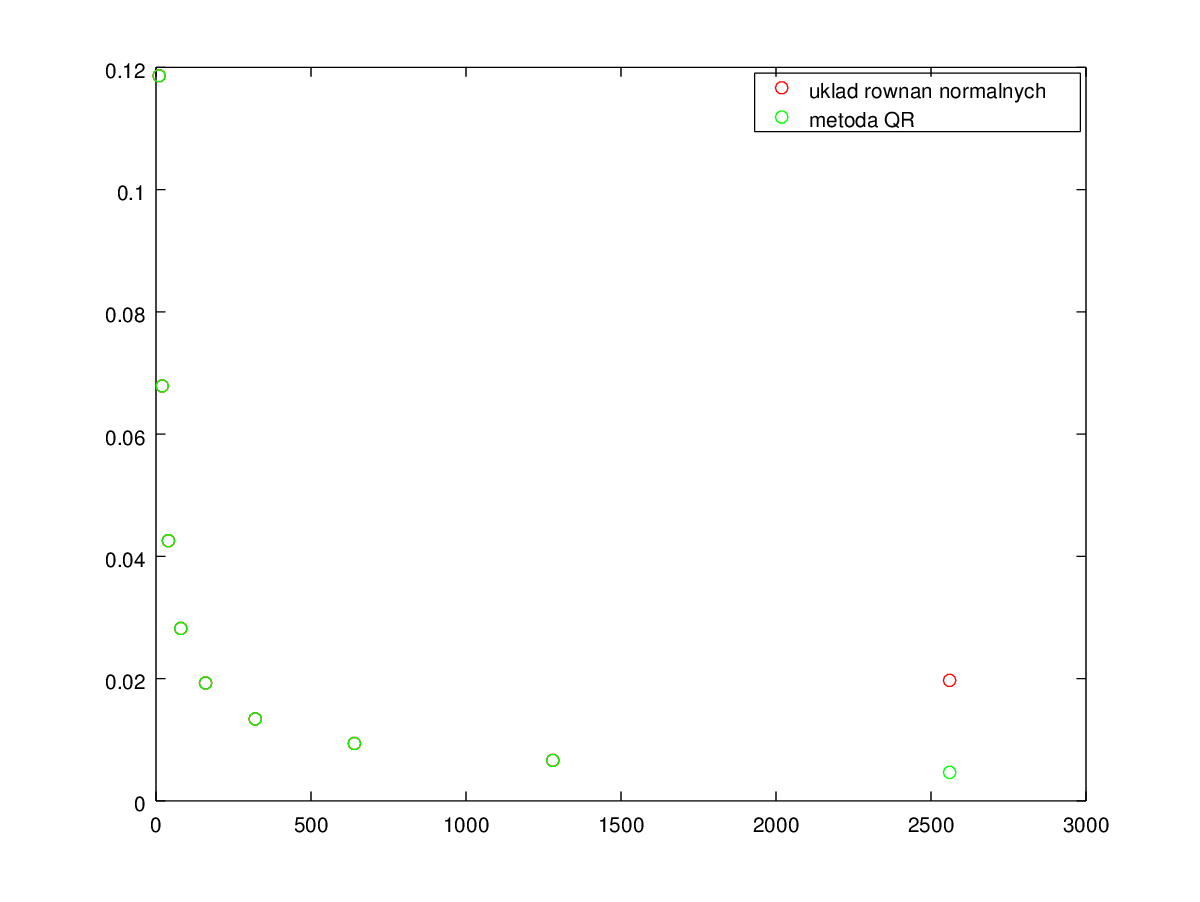
\includegraphics[width=\textwidth]{figure1}
\end{figure}

\begin{figure}[th]
\caption{Podpunkt 2}
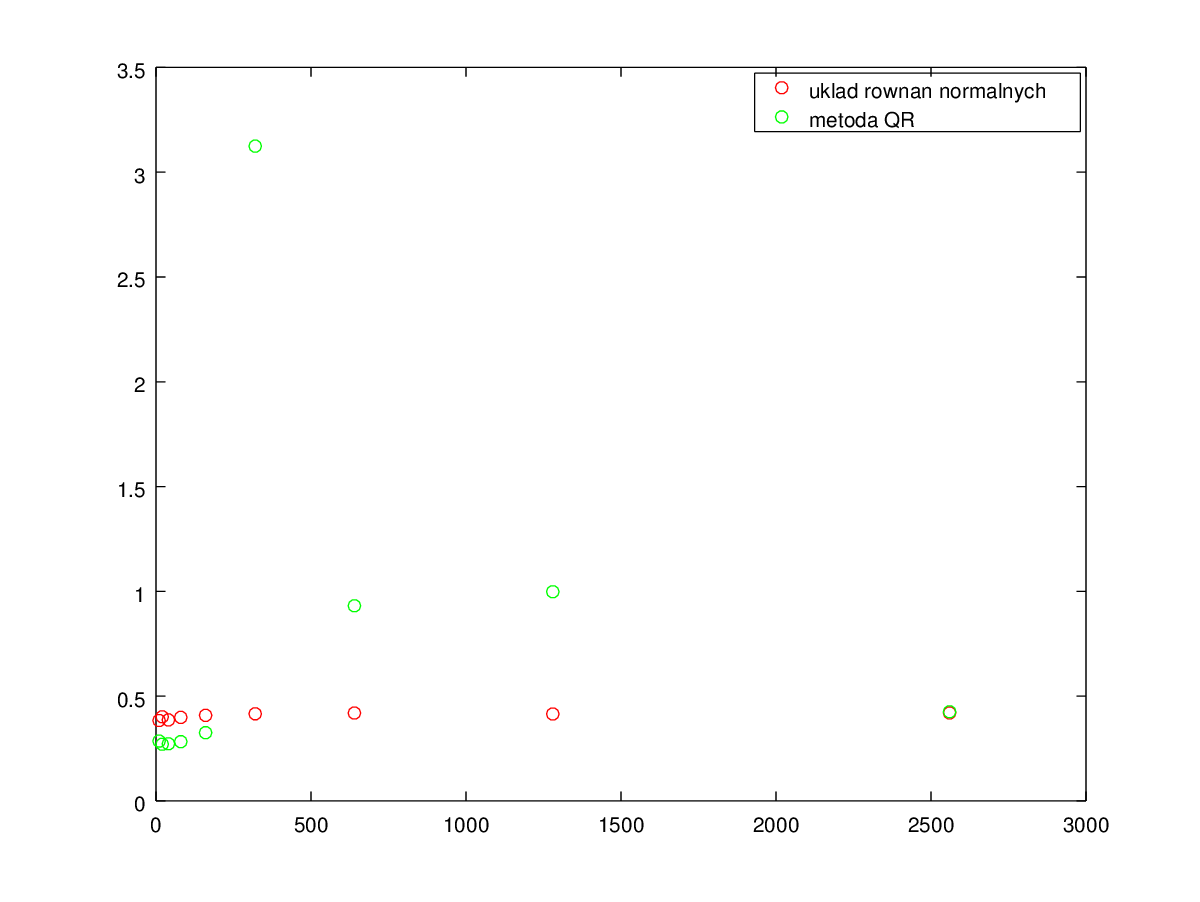
\includegraphics[width=\textwidth]{figure2}
\end{figure}


\vspace{10cm}
\subsection{Wnioski}
Jak wynika z wykresu dla podpunktu 1 rozwiązania dla obu metod w większości się pokrywają. Jest to spowodowane dobrym uwarunkowaniem macierzy dla obu metod. Natomiast w podpunkcie 2 metoda QR dokładniej wyznacza rozwiązania 
jednak tylko dla pewniej liczby równań. Jest to spowodowane złym uwarunkowaniem dla obu algorytmów. Wyniki nie spełniają żadnej znanej zależności, szczególnie w przypadku metody QR ponieważ większa ilość operacji uwydatnia błędy. 
	
\end{document}


